\chapter{Analysis}\label{analysis}

\section{Allocating Computationl Kernels for Performance}
\subsection{Allocating Based on Only Forward Pass Analysis}
When computing an optimal allocation of kernels to the fully-connected layers, it was enough to account only for the forward pass. This is because in the backward pass, there are 2 times the kernel is used, during previous layer neuron gradient calculation, and during weight gradient calculation. In each case, the amount of multiplications is equal to the sum of the fan-ins of all the neurons. For the forward pass, every neuron receives an input from every neuron in the previous layer, so the amount of MACs will be:
\begin{align}
MACs = \text{\#previous layer neurons} \times \text{\#current layer neurons} \label{macs}
\end{align}

For the backward pass, each backpropagated neuron gradient to a previous layer requires an MAC on all the neurons in the current layer. This must be done for each neuron in the previous layer, thus the total amount of MACs for backpropagating neuron gradients is also equivalent to Equation \ref{macs}.

For computing all the weight gradients in a layer, every weight for every neuron must be multiplied by a gradient. Each neuron in the current layer will have a \# previous layer neurons weights, as that is the fan-in for each neuron. Thus, there same amount of multiplications is also equal to the expresion in Equation \ref{macs}.

The backward pass also has a weight updating step, however, this uses bitshifts and not DSP slices to multiply the weight gradient by the learning rate. As such, the backward pass in this model uses exactly twice the amount of multiplications as the forward pass, so the optimal allocation of kernels is optimal for both the forward and backward pass. Note however, that even if the update step used multiplication, the amount of extra multiplications would be 1 for every weight, which would still be a multiple of the amount of multiplciations in the forward pass.

\subsection{Distribution of the Kernels}
Table \ref{macs-per-layer} shows the fan-in, number of neurons, and thus the number of MACs per layer during the forward pass. 
\begin{table}
	\centering
	\begin{tabular}{|l|l|l|l|}
		\hline
		Layer & Fan-in per Neuron & \# Neurons & MACs \\\hline 
		FC0 & 784  & 98 & 76832 \\\hline 
		FC1 & 98 & 64 & 6272 \\\hline 
		FC2 & 64 & 10 & 640 \\\hline
	\end{tabular}
	\caption{MACs per layer during the forward pass}
	\label{macs-per-layer}
\end{table}

Furthermore, recall that a kernel operates on only 1 neuron at a time. Therefore, the amount of kernels allocated should be either a multiple or a factor of the amount of neurons such that work can be evenly distributed across the kernels. Given the 220 DSP slices on the FPGA, this becomes an optimization problem such that the amount of time for each layer to finish computing their outputs should be roughly the same. This would allow for pipelined input processing if offline training for large batch-sizes were to be implemented.

FC0 has 120.05 times more MACs than FC2. FC1 has 9.8 times more MACs than FC2. To balance runtime per layer, FC0 should then have roughly 120.05 times more DSPs than FC2 and so on. Using this information, we can write an equation for the amount of MACs and use substitution to come up with an ideal allocation scheme if allocate partial DSPs and ignore the fact that kernels work on 1 neuron at a time.
\begin{align}
	\text{DSP}_{FC0} &= 120.05 {DSP}_{FC2} \label{mac-1}\\	
	\text{DSP}_{FC1} &= 9.8 {DSP}_{FC2} \label{mac-2}\\
	\text{\# DSPs} &= 220 = \text{DSP}_{FC0} + \text{DSP}_{FC1} + \text{DSP}_{FC2} \label{mac-3}\\	
	\intertext{Substituting into equation \ref{mac-3} using equations \ref{mac-1} and \ref{mac-2}:}\\
	220 &= 120.05 {DSP}_{FC2} + 9.8  {DSP}_{FC2} +  {DSP}_{FC2} \\
	220 &= 129.85 {DSP}_{FC2}\\ 
	{DSP}_{FC2} &= 1.69 \label{mac-4}\\
	\intertext{Substituting the result from \ref{mac-4} into equations \ref{mac-1} and \ref{mac-2}:}
	\text{DSP}_{FC0} &= 120.05 \times 1.60 = 203.36\label{mac-5}\\	
	\text{DSP}_{FC1} &= 9.8 \times 1.69 = 16.60\label{mac-6}	
\end{align}
Thus if the 220 DSPs could be divided up ignoring all previous restrictions, the DSPs should be allocated according to Equations \ref{mac-4}, \ref{mac-5} and \ref{mac-6}. However, this is not possible, and DSPs are indivisible and the amount of kernels per layer should be a factor or multiple of the number of neurons, but it provides an maximum upper bound for performance.

Starting with layer FC0, which has 98 neurons, we should delegate 196 kernels. This is quite close to the optimal 203.36 computed above, thus layer FC0 should be allocated 196 kernels, which is $\frac{196}{203.36} = 96.38\%$ of the maximum upper bound. Continuing to layer FC1, which has 64 neurons, the optimal allocation is 16.6. The closest factor of 64 is thus 16 so 16 kernels are allocated, resulting in the same computation time as FC0 with $\frac{16}{16.6} = 96.38\%$ of the upper bound. Finally, layer FC2, with 10 neurons, rounding down and allocating 1 kernel would result in only $\frac{1}{1.69} = 59.17\%$ of the upper bound performance. Since a few kernels were freed up a from rounding down in FC0 and FC1, FC2 could be allocated 2 kernels, which allows it to finish faster than the optimally balanced latency for the 3 layers.

The final allocation of kernels is shown in Table \ref{dsp-allocat}. A pipelined solution is only as fast as its slowest step. Since FC0 and FC1 is the farthest away from the optimal upper bound, this solution performs at 96.38\% of the theoretical upper bound for performance. It is worth re-mentioning that this upper bound is not actually possible since it assumes DSPs as divisible and that kernels can arbitrarily switched from neuron to neuron mid-computation, which would require finer-parallelism than what is supported in this architecture. Also note that since 214 of the 220 DSPs are used, the softmax layer was also able to use a DSP for calculation of the exponential function.

\begin{table}
	\centering 
	\begin{tabular}{|l|l|}
		\hline 
		Layer & \# Kernels \\\hline
		FC0 & 196 \\\hline
		FC1 & 16 \\\hline
		FC2 & 2	\\\hline
		Total & 214	\\\hline
	\end{tabular}
	\caption{Kernel allocation between the fully-connected layers.}
	\label{dsp-allocat}
\end{table}

\section{Cycle Analysis}
This section calculates the computational cycles required for computing the forward and backward passes. Cycles spent pipelining or performing non-computational work are not included in this analysis. $FP$ and $BP$ are the amount of cycles needed to compute the forward pass and backward pass respectively. The amount of cycles for fully-connected layers in the forward pass can be roughly represented by $\frac{\# \text{MACs}}{\# \text{kernels}}$.
\begin{align}
	FP_{FC0} = \frac{76832}{196} &= 392\text{ cycles}\\	
	FP_{FC1} = \frac{6272}{16} &= 392 \text{ cycles}\\
	FP_{FC2} = \frac{640}{2} &= 320 \text{ cycles}	
\end{align}
For the softmax layer, there are several computational steps. For simplicity, conversions from fixed to floating point and vice versa are not included nor is the max circuit and the subsequent subtraction of the max. The softmax forward pass perform the exponential function, a sum of 10 values, and then a fixed point divison. The exponential function requires 20 cycles, the summation requires 10 cycles and the dividor takes 46 cycles. This results in $FP_{softmax} = 20 + 10 + 46 = 76$ cycles. $FP$ is computed in Equation \ref{fp-cycles}.
\begin{align}
	FP &= FP_{FC0} + FP_{FC1} + FP_{FC2} + FP_{softmax} \\
	FP &= 392 + 392 + 320 + 76\\
	FP &= 1180	 \text{ cycles} \label{fp-cycles}
\end{align}

Computing the backward pass is a bit more involved. Note that backpropagation of from the softmax layer to FC2 takes 1 cycle so it is not included. Each fully-connected layer first backpropagates neuron gradients for the previous layer and then computes the weight gradients, however, the previous layer can start computing the backward pass as soon as the neuron gradients are ready. Thus, the time for backpropagation to finish is not based on layer computation time, but instead $BP$ can be calculated by using neuron gradient computation time. Recall that the amount of computational cycles required to perform  backpropagation of neuron gradients ($NG$) and computation of weight gradients ($WG$) is the same. As described in Chapter \ref{hw-model}, updating the weights ($UW$) requires 2 cycles per-weight rather than 1-cycle per weight. Thus the $UW$ step requires twice as many cycles as the others. The longest path during backpropagation is thus backpropagating neuron gradients from FC2 to FC1, from FC1 to FC0 and then performing $WG$ in FC0 followed by $UW$.
\begin{align}
	BP &= NG_{FC2} + NG_{FC1} + WG_{FC0} + UW_{FC0} \\
	\intertext{Substituting the forward pass cycles for the layers, as they are equivalent: }
	BP &= 320 + 392 + 392 + (2 \times 392)\\
	BP &= 1888\label{bp-cycles}
	\intertext{Thus, the amount of cycles spent performing computation during 1 training cycle is: }
	\text {Cycles } &= FP + BP = 1180 + 1888 \\
	\text {Cycles } &= 3068 \text{ cycles}
\end{align} 

This analysis has shown that the forward pass has 1,180 cycles of computation, and that one iteration of training contains 3,068 cycles of computation. Indeed, by viewing the output simulation file, this is confirmed as the forward pass finishes at cycle at cycle 1,235 and the training iteration concludes at cycle 3,145. The discrepancy in simulated cycles to computational cycles comes from the overhead of  other actions in the design such as a max circuit, a pipelined addition reduction for neuron gradients, buffering of data between layers, non-computational data pipelining in layers, and floating-fixed type conversions. With a clock period of 20 nanoseconds (50 MHz) and ignoring data transfer overhead and delay, this would mean that 1 training iteration should take: $3145 \times 20ns = 62900 ns$ or approximately 62.9 microseconds.

This result can be compared with the experimental results achieved. One training epoch was measured to take 5.455 seconds, as shown in Figure \ref{train-runtime-res}. Using the above calculated cycle results, at 62.9 microseconds per training iteration, training over a 60,000 image dataset we have:
\begin{align}
	t &= 62.9\text{e}^{-6} \times 60000 = 3.774 \text{ seconds}\\
	\intertext{Recall however, how the active cycle percentage during training was only 69.2\%. Thus, the analytically derived computation time should account for this: }
	t &= 3.774 \times \frac{1.0}{0.692}\\
	t &= 5.454 \text{ seconds}
\end{align}
Compared to the experimentally measured epoch time of 5.455 seconds, the analytically computed training time of 5.454 seconds using cycle analysis is nearly exactly the same. The experimental data has thus successfully validated the cycle analysis.

\section{Improving Performance}
As was shown in Table \ref{active-cycle-table} of the results section, the active cycle percentage for training is only 69.20\%. Thus the first step to improve runtime performance would be to make data available for the FPGA to process faster. A suggested approach would be to use DRAM to stream data to the FPGA as done in other projects such as the neural network inference hardware accelerator proposed by Qiao et. al \cite{qiao}.

If an active cycle percentage of near 100\% can be achieved from doing this, the next step to would be to optimize performance on the FPGA. The quickest route to doing this would be to improve the clock frequency. The design was clocked at a relatively low-frequency since it was not the bottleneck for performance. As such, the clock frequency was not investigated heavily during the design of the FPGA architecture, since improving this clock frequency would only increase the amount of time that the layers in the FPGA spend idling.

\section{Granularity for Neural Network Computation}
A key difference between training using this accelerator and training using GPUs is that this accelerator uses a much more fine-grained level of parallelism. While GPUs use data-level parallelism, this design uses neuron-level parallelism. Some attempts  have been made to implement finer-level parallelism training on GPUs by Jiang et. al, though only yielded modest improvements of 1.58 to 2.19 times the speedup \cite{fine-grained-gpu}. 

As a result, if one were to use the PyGPU solution to perform online training, then the GPU is 2.95 times slower than the CPU solution, which was 17.35 times slower than the hardware model (results in \cite[inline]{Experiment results appendix}). Therefore, for online training, using fine-grained parallelism at the neuron level is the only place to find speedup, as data-level parallelism is not possible during online training where the batch size is only 1.

\section{Ideal Learning Rate vs. Precision}
One of the key intricacies in optimizing hyperparameters for the training process was balancing an ideal learning rate against increased precision error. Normally one need not think about precision when choosing a learning rate. However, in this accelerator, choosing what perhaps would be a more ideal learning rate might actually induce higher training error if it is too small since a smaller learning rate means fewer bits of gradient data are kept. For this project, this is compounded even further by the general notion that online training performs best with smaller learning rates. 

For example, a learning rate of 0.001 results in a much better solution than a learning rate of 0.016 when a batch size of 1 is used for the implemented network architecture. However, the smaller in the implemented accelerator, this would mean an additional 4 bitshifts to the right when updating the weights. This results in a weight update that will have 4 fewer bits of information. In this project, the best training solution was found using 9 bitshifts to the right, or a learning rate of 0.00195. The weight gradients in this project are of number format Q1.17. Shifting this to the right 9 bits results in a Q1.8 number. This means that each and every weight update in the network only have 8 bits of information.

\paragraph{Vanishing Gradient Problem}
To add on even further to the aforementioned loss of information is that many of the gradients are already quite small. This is largely in part to a phenomenon referred to as the vanishing gradient problem. The vanishing gradient problem in neural networks refers to the fact that as one backpropagates further and further through the network, the gradients become smaller and smaller. To illustrate this phenomenon, the distributions of non-zero gradients in the implemented network has been plotted in Figure \ref{weight-distrib}. As can be seen from the figure, gradients become smaller as backpropagation progresses from FC2 to FC0. Thus, as the gradients become smaller, they also become harder to represent using the limited precision of the hardware model. In an architecture where many bits of information are already being lost due to the learning rate, the vanishing gradient problem exacerbates the precision-induced error during training even more.

\begin{figure}
	\centering 
	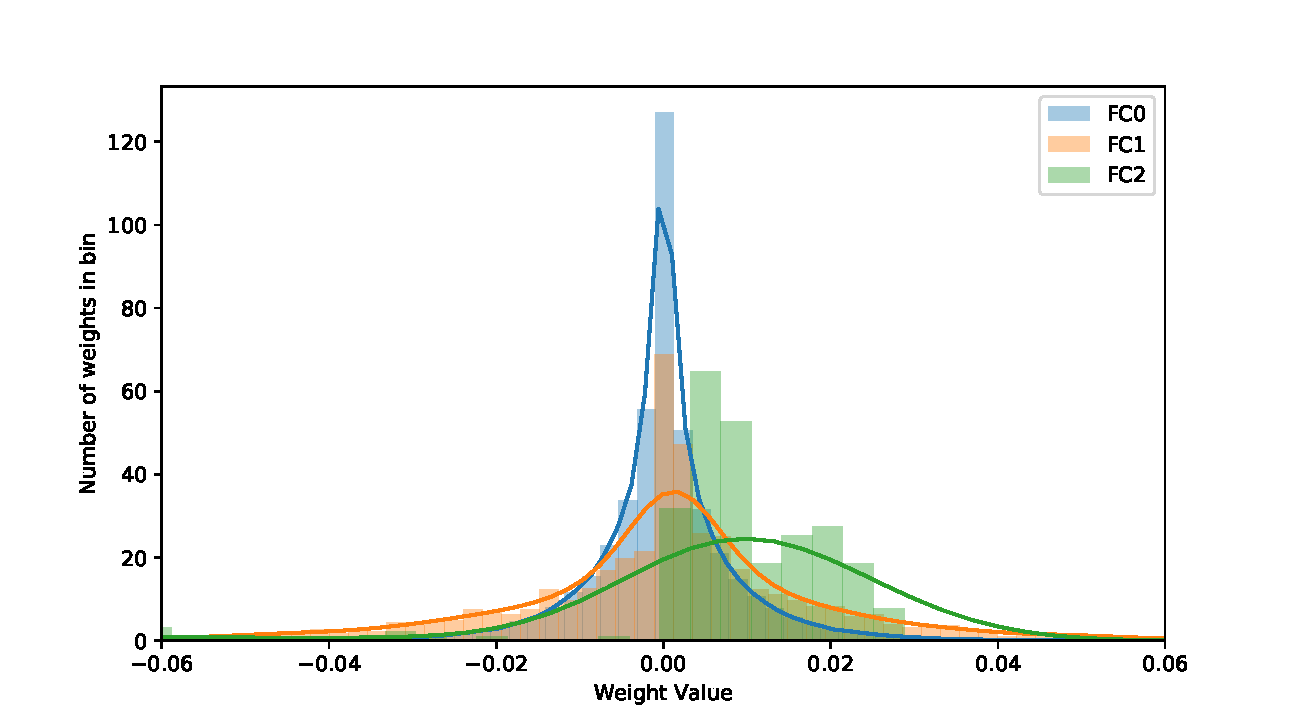
\includegraphics[width=\textwidth]{figures/weight_distrib}
	\caption{Weight gradient distribution for the 3 fully-connected layers after performing a single backward pass on the network using the input used to verify the hardware model from Chapter \ref{hw-model-testing}.}
	\label{weight-distrib}
\end{figure}

\section{Potential Solutions for the Lack of Precision}
As 18-bit fixed-point computation has been shown to be too imprecise to perform training on this network, potential solutions to this problem should be observed. It is the author's opinion that future accelerators for the training of neural networks would be best implemeneted by using 32-bit floating point as was done in the F-CNN accelerator by Zhao et. al \cite{FCNN}. 

However, if 32-bit floating point is infeasible, or if accuracy is to be traded off for improved speed, area, and storage of weights, then investigations into designing accelerators using 16-bit or 24-bit floating-point computation could be made.

If the architecture must use fixed point, then the author would suggest first investigating 32-bit fixed-point computation with varying radices. If storage restrictions permit and the design performs multiplications using DSP slices, then a maximum of 36 bits would be supported for completing a multiplication using 2 DSPs in 1 cycle. This stems from the fact that 18 bits is the maximum width for one of the ports in a DSP-multiply. Otherwise, multiplication could also be a multi-cycle computation to trade off time for improved precision.

\section{Weight Storage}
The implemented neural network was specifically designed such that the weights and weight gradients could fit in the BRAM. Since 76.79\% of the BRAM was utilized, the implemented network is representative of what architectures may be supported in BRAM as it comes close to hitting the upper limit of network size that can be supported entirely using BRAM. For networks larger than the implemented neural network for this thesis, other solutions such as a streaming weight and weight gradient datapath to DRAM would be required. 

In addition, since the precision of the weight and weight gradients in this project proved to be inadequate for convergence to a local optimum during training, it should be noted that increasing precision would also increase BRAM utilization. This network would be able to use a maximum of 23-bits of precision for the weights while still fitting into BRAM at roughly 98.12\% utilization. If more bits are needed for successful training then the network architecture would have to be made smaller or the hardware architecture would need to use a streaming datapath solution.
